\renewcommand{\theequation}{\theenumi}
\begin{enumerate}[label=\thesection.\arabic*.,ref=\thesection.\theenumi]
\numberwithin{equation}{enumi}
\item The figure for A quadrilateral obtained in the question looks like Fig. \ref{fig:quad}.
with side $a$, $c$, $e$ and $d$.
\\
%\renewcommand{\thefigure}{\theenumi.\arabic{figure}}
\begin{figure}[!ht]
\centering
\resizebox{\columnwidth}{!}{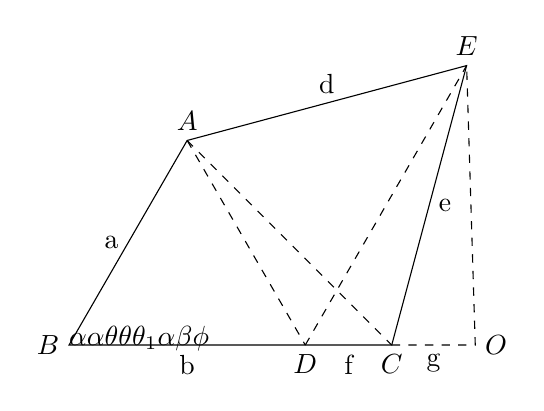
\begin{tikzpicture}
%Marking coordiantes

\coordinate [label=above:$A$] (A) at (1.5,2.59807621);
\coordinate [label=left:$B$] (B) at (0,0);
\coordinate [label=below:$C$] (C) at (4.09807621,0);
\coordinate [label=below:$D$] (D) at (3,0);
\coordinate [label=above:$E$] (E) at (5.04903811,3.54903811);
\coordinate [label=right:$O$] (O) at (5.15873638,0);

%Drawing quadrilaterl ABCE
\draw (A) -- node[left] {$\textrm{a}$} (B) -- node[below] {$\textrm{b}$} (D) -- node[below] {$\textrm{f}$} (C) -- node[right] {$\textrm{e}$} (E) -- node[above] {$\textrm{d}$} (A);
\draw[dashed] (D) -- (E);
\draw[dashed] (A) -- (D);
\draw[dashed] (C) -- node[below] {$\textrm{g}$} (O) -- (E);
\draw[dashed] (A) -- (C);

%Drawing and marking angles
\tkzMarkRightAngle[size=0.2](E,O,C)

\tkzMarkAngle[fill=orange!50,size=0.5cm,mark=](D,B,A)
\tkzLabelAngle[pos=0.7](D,B,A){$\alpha$}

\tkzMarkAngle[fill=orange!40,size=0.5cm,mark=](A,D,B)
\tkzLabelAngle[pos=0.7](A,D,B){$\alpha$}

\tkzMarkAngle[fill=orange!40,size=0.5cm,mark=](B,A,D)
\tkzLabelAngle[pos=0.7](B,A,D){$\theta$}

\tkzMarkAngle[fill=orange!40,size=0.5cm,mark=](C,A,E)
\tkzLabelAngle[pos=0.7](C,A,E){$\theta$}

\tkzMarkAngle[fill=orange!40,size=0.5cm,mark=](O,C,E)
\tkzLabelAngle[pos=0.7](O,C,E){$\theta _1$}

\tkzMarkAngle[fill=orange!40,size=0.5cm,mark=](E,C,A)
\tkzLabelAngle[pos=0.7](E,C,A){$\alpha$}

\tkzMarkAngle[fill=orange!40,size=0.5cm,mark=](A,C,B)
\tkzLabelAngle[pos=0.7](A,C,B){$\beta$}

\tkzMarkAngle[size=1.1cm,mark=](D,A,C)
\tkzLabelAngle[pos=1.3](D,A,C){$\phi$}

\end{tikzpicture}}
\caption{Quadrilateral ABCE by Latex-Tikz}
\label{fig:quad}	
\end{figure}
%
%
%\renewcommand{\thefigure}{\theenumi}
%
\item List the design parameters for construction
\label{const:table1}
\\
\solution See Table. \ref{table:table1}. 
%
\begin{table}[ht!]
\centering
%%%%%%%%%%%%%%%%%%%%%%%%%%%%%%%%%%%%%%%%%%%%%%%%%%%%%%%%%%%%%%%%%%%%%%
%%                                                                  %%
%%  This is the header of a LaTeX2e file exported from Gnumeric.    %%
%%                                                                  %%
%%  This file can be compiled as it stands or included in another   %%
%%  LaTeX document. The table is based on the longtable package so  %%
%%  the longtable options (headers, footers...) can be set in the   %%
%%  preamble section below (see PRAMBLE).                           %%
%%                                                                  %%
%%  To include the file in another, the following two lines must be %%
%%  in the including file:                                          %%
%%        \def\inputGnumericTable{}                                 %%
%%  at the beginning of the file and:                               %%
%%        \input{name-of-this-file.tex}                             %%
%%  where the table is to be placed. Note also that the including   %%
%%  file must use the following packages for the table to be        %%
%%  rendered correctly:                                             %%
%%    \usepackage[latin1]{inputenc}                                 %%
%%    \usepackage{color}                                            %%
%%    \usepackage{array}                                            %%
%%    \usepackage{longtable}                                        %%
%%    \usepackage{calc}                                             %%
%%    \usepackage{multirow}                                         %%
%%    \usepackage{hhline}                                           %%
%%    \usepackage{ifthen}                                           %%
%%  optionally (for landscape tables embedded in another document): %%
%%    \usepackage{lscape}                                           %%
%%                                                                  %%
%%%%%%%%%%%%%%%%%%%%%%%%%%%%%%%%%%%%%%%%%%%%%%%%%%%%%%%%%%%%%%%%%%%%%%



%%  This section checks if we are begin input into another file or  %%
%%  the file will be compiled alone. First use a macro taken from   %%
%%  the TeXbook ex 7.7 (suggestion of Han-Wen Nienhuys).            %%
\def\ifundefined#1{\expandafter\ifx\csname#1\endcsname\relax}


%%  Check for the \def token for inputed files. If it is not        %%
%%  defined, the file will be processed as a standalone and the     %%
%%  preamble will be used.                                          %%
\ifundefined{inputGnumericTable}

%%  We must be able to close or not the document at the end.        %%
	\def\gnumericTableEnd{\end{document}}


%%%%%%%%%%%%%%%%%%%%%%%%%%%%%%%%%%%%%%%%%%%%%%%%%%%%%%%%%%%%%%%%%%%%%%
%%                                                                  %%
%%  This is the PREAMBLE. Change these values to get the right      %%
%%  paper size and other niceties.                                  %%
%%                                                                  %%
%%%%%%%%%%%%%%%%%%%%%%%%%%%%%%%%%%%%%%%%%%%%%%%%%%%%%%%%%%%%%%%%%%%%%%

	\documentclass[12pt%
			  %,landscape%
                    ]{report}
       \usepackage[latin1]{inputenc}
       \usepackage{fullpage}
       \usepackage{color}
       \usepackage{array}
       \usepackage{longtable}
       \usepackage{calc}
       \usepackage{multirow}
       \usepackage{hhline}
       \usepackage{ifthen}

	\begin{document}


%%  End of the preamble for the standalone. The next section is for %%
%%  documents which are included into other LaTeX2e files.          %%
\else

%%  We are not a stand alone document. For a regular table, we will %%
%%  have no preamble and only define the closing to mean nothing.   %%
    \def\gnumericTableEnd{}

%%  If we want landscape mode in an embedded document, comment out  %%
%%  the line above and uncomment the two below. The table will      %%
%%  begin on a new page and run in landscape mode.                  %%
%       \def\gnumericTableEnd{\end{landscape}}
%       \begin{landscape}


%%  End of the else clause for this file being \input.              %%
\fi

%%%%%%%%%%%%%%%%%%%%%%%%%%%%%%%%%%%%%%%%%%%%%%%%%%%%%%%%%%%%%%%%%%%%%%
%%                                                                  %%
%%  The rest is the gnumeric table, except for the closing          %%
%%  statement. Changes below will alter the table's appearance.     %%
%%                                                                  %%
%%%%%%%%%%%%%%%%%%%%%%%%%%%%%%%%%%%%%%%%%%%%%%%%%%%%%%%%%%%%%%%%%%%%%%

\providecommand{\gnumericmathit}[1]{#1} 
%%  Uncomment the next line if you would like your numbers to be in %%
%%  italics if they are italizised in the gnumeric table.           %%
%\renewcommand{\gnumericmathit}[1]{\mathit{#1}}
\providecommand{\gnumericPB}[1]%
{\let\gnumericTemp=\\#1\let\\=\gnumericTemp\hspace{0pt}}
 \ifundefined{gnumericTableWidthDefined}
        \newlength{\gnumericTableWidth}
        \newlength{\gnumericTableWidthComplete}
        \newlength{\gnumericMultiRowLength}
        \global\def\gnumericTableWidthDefined{}
 \fi
%% The following setting protects this code from babel shorthands.  %%
 \ifthenelse{\isundefined{\languageshorthands}}{}{\languageshorthands{english}}
%%  The default table format retains the relative column widths of  %%
%%  gnumeric. They can easily be changed to c, r or l. In that case %%
%%  you may want to comment out the next line and uncomment the one %%
%%  thereafter                                                      %%
\providecommand\gnumbox{\makebox[0pt]}
%%\providecommand\gnumbox[1][]{\makebox}

%% to adjust positions in multirow situations                       %%
\setlength{\bigstrutjot}{\jot}
\setlength{\extrarowheight}{\doublerulesep}

%%  The \setlongtables command keeps column widths the same across  %%
%%  pages. Simply comment out next line for varying column widths.  %%
\setlongtables

\setlength\gnumericTableWidth{%
	56pt+%
	33pt+%
0pt}
\def\gumericNumCols{2}
\setlength\gnumericTableWidthComplete{\gnumericTableWidth+%
         \tabcolsep*\gumericNumCols*2+\arrayrulewidth*\gumericNumCols}
\ifthenelse{\lengthtest{\gnumericTableWidthComplete > \linewidth}}%
         {\def\gnumericScale{\ratio{\linewidth-%
                        \tabcolsep*\gumericNumCols*2-%
                        \arrayrulewidth*\gumericNumCols}%
{\gnumericTableWidth}}}%
{\def\gnumericScale{1}}

%%%%%%%%%%%%%%%%%%%%%%%%%%%%%%%%%%%%%%%%%%%%%%%%%%%%%%%%%%%%%%%%%%%%%%
%%                                                                  %%
%% The following are the widths of the various columns. We are      %%
%% defining them here because then they are easier to change.       %%
%% Depending on the cell formats we may use them more than once.    %%
%%                                                                  %%
%%%%%%%%%%%%%%%%%%%%%%%%%%%%%%%%%%%%%%%%%%%%%%%%%%%%%%%%%%%%%%%%%%%%%%

\ifthenelse{\isundefined{\gnumericColA}}{\newlength{\gnumericColA}}{}\settowidth{\gnumericColA}{\begin{tabular}{@{}p{56pt*\gnumericScale}@{}}x\end{tabular}}
\ifthenelse{\isundefined{\gnumericColB}}{\newlength{\gnumericColB}}{}\settowidth{\gnumericColB}{\begin{tabular}{@{}p{33pt*\gnumericScale}@{}}x\end{tabular}}

\begin{tabular}[c]{%
	b{\gnumericColA}%
	b{\gnumericColB}%
	}

%%%%%%%%%%%%%%%%%%%%%%%%%%%%%%%%%%%%%%%%%%%%%%%%%%%%%%%%%%%%%%%%%%%%%%
%%  The longtable options. (Caption, headers... see Goosens, p.124) %%
%	\caption{The Table Caption.}             \\	%
% \hline	% Across the top of the table.
%%  The rest of these options are table rows which are placed on    %%
%%  the first, last or every page. Use \multicolumn if you want.    %%

%%  Header for the first page.                                      %%
%	\multicolumn{2}{c}{The First Header} \\ \hline 
%	\multicolumn{1}{c}{colTag}	%Column 1
%	&\multicolumn{1}{c}{colTag}	\\ \hline %Last column
%	\endfirsthead

%%  The running header definition.                                  %%
%	\hline
%	\multicolumn{2}{l}{\ldots\small\slshape continued} \\ \hline
%	\multicolumn{1}{c}{colTag}	%Column 1
%	&\multicolumn{1}{c}{colTag}	\\ \hline %Last column
%	\endhead

%%  The running footer definition.                                  %%
%	\hline
%	\multicolumn{2}{r}{\small\slshape continued\ldots} \\
%	\endfoot

%%  The ending footer definition.                                   %%
%	\multicolumn{2}{c}{That's all folks} \\ \hline 
%	\endlastfoot
%%%%%%%%%%%%%%%%%%%%%%%%%%%%%%%%%%%%%%%%%%%%%%%%%%%%%%%%%%%%%%%%%%%%%%

\hhline{|-|-}
	 \multicolumn{1}{|p{\gnumericColA}|}%
	{\gnumericPB{\centering}\gnumbox{Parameter}}
	&\multicolumn{1}{p{\gnumericColB}|}%
	{\gnumericPB{\centering}\gnumbox{Value}}
\\
\hhline{|--|}
	 \multicolumn{1}{|p{\gnumericColA}|}%
	{\gnumericPB{\centering}\gnumbox{$a$}}
	&\multicolumn{1}{p{\gnumericColB}|}%
	{\gnumericPB{\centering}\gnumbox{3}}
\\
\hhline{|--|}
	 \multicolumn{1}{|p{\gnumericColA}|}%
	{\gnumericPB{\centering}\gnumbox{$\angle{BAD}$}}
	&\multicolumn{1}{p{\gnumericColB}|}%
	{\gnumericPB{\centering}\gnumbox{60\degree}}
\\
\hhline{|-|-|}
\end{tabular}

\ifthenelse{\isundefined{\languageshorthands}}{}{\languageshorthands{\languagename}}
\gnumericTableEnd

\caption{To construct quadrilaterl $ABCE$}
\label{table:table1}	
\end{table}
\item Find the coordinates of the various points in Fig. \ref{fig:quad}
\label{const:quad}
\\
%
\solution From the given information, 
\begin{align}
\label{eq:constr_a}
\vec{A} &= \myvec{p\\q} 
\\
\vec{B} &= \myvec{0\\0}, 
\label{eq:constr_b}
\\
\vec{C} &= \myvec{c\\0}
\label{eq:constr_c}
\\
\vec{D} &= \myvec{b\\0}
\label{eq:constr_d}
\\
\vec{E} &= \myvec{r\\s}
\label{eq:constr_e}
\end{align}

\textbf{For Vertices A}
\\
\begin{equation} \label{eq:one}
AB={\Vert A-B \Vert}^2={\Vert A\Vert}^2=a^2
\end{equation}

\begin{equation}
DB={\Vert D-B \Vert}^2={\Vert D\Vert}^2=b^2
\end{equation}

\begin{equation} \label{eq:two}
AD={\Vert A-D \Vert}^2=a^2
\end{equation}
\\
Solving equation \ref{eq:two}\\
$a^2=A^TA+D^TD-A^TD-D^TA$\\
$a^2={\Vert A\Vert}^2+{\Vert D\Vert}^2-2A^TD$\\
$a^2=a^2+b^2-2pb$\\
\begin{equation}
p=\frac{b^2+a^2-a^2}{2b}=\frac{b^2}{2b}=\frac{b}{2}
\end{equation}
\\
From equation \ref{eq:one}
\\
$\Vert A \Vert =a^2= p^2+q^2$\\
\begin{equation}
q=\pm \sqrt{a^2-p^2}
\end{equation}
\\
\textbf{For Vertices E}\\
If we draw perpendicular line from E, it meets on x-axis at point O.\\
Consider $OC =g$
Then, 
\begin{equation}
cos \theta _1 = \frac{OC}{EC}=\frac{g}{e}
\end{equation}

\begin{equation}
g = e cos\theta _1
\end{equation}
\begin{equation}
tan\theta _1=\frac{OE}{OC}=\frac{h}{g}
\end{equation}

\begin{equation}
h=gtan \theta _1
\end{equation}

\begin{equation}
r = c+g
\end{equation}
\begin{equation}
s = h
\end{equation}

The values are listed in 
%\item List the  derived values.
%\label{const:table2}
%\\
%\solution See  
Table. \ref{table:table2} 
\begin{table}[ht!]
\centering
\begin{tabular}{ |p{3cm}|p{3cm}|  }
\hline
 \multicolumn{2}{|c|}{Derived Values.} \\
\hline
$\vec{A}$ & $$\begin{pmatrix}1.5\\2.6\end{pmatrix}$$\\					
\hline
$\vec{C}$ & $$\begin{pmatrix}4.1\\0\end{pmatrix} $$\\
\hline
$\vec{E}$ & $$\begin{pmatrix}5.05\\3.55\end{pmatrix} $$\\
\hline
\end{tabular}
\caption{To construct $ABCE$}
\label{table:table2}
\end{table}
%
\item Draw Fig. \ref{fig:quad}.	
\\
\solution The  following Python code generates Fig. \ref{fig:quad}
%
\begin{lstlisting}
codes/quadrilateral.py
\end{lstlisting}
\begin{figure}[!ht]
\centering
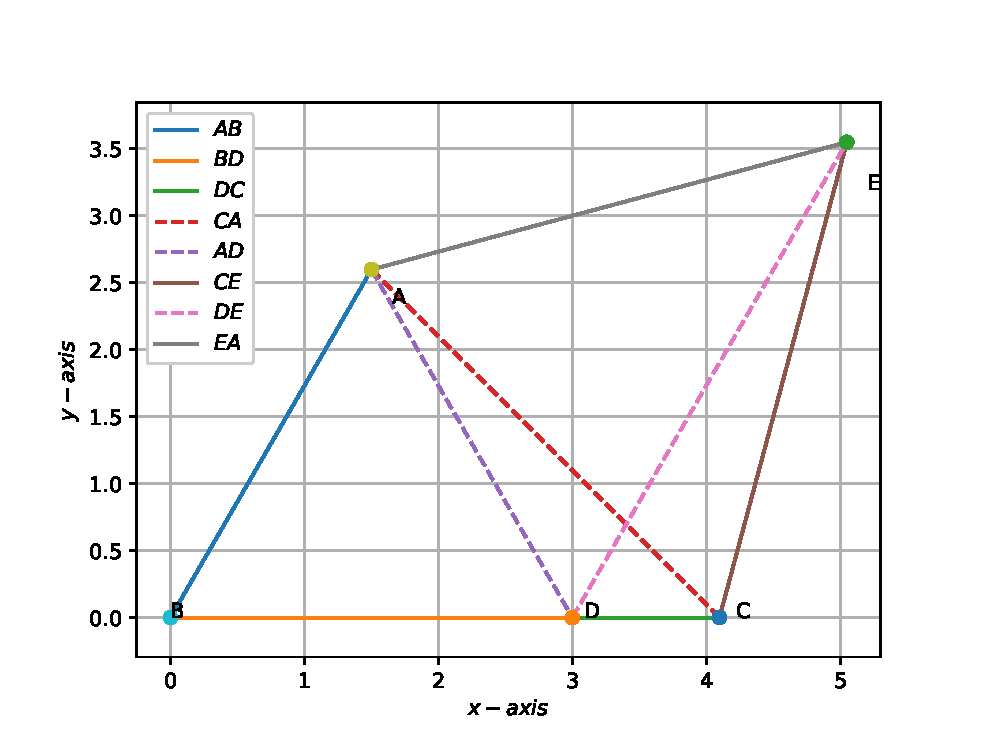
\includegraphics[width=\columnwidth]{./figs/quadrilateral.eps}
\caption{Quadrilateral generated using python}
\label{fig:quad_py}
\end{figure}

%
and the equivalent latex-tikz code generating Fig. \ref{fig:quad_py} is 
\begin{lstlisting}
figs/quadrilateral.tex
\end{lstlisting}
%
The above latex code can be compiled as a standalone document as
\begin{lstlisting}
figs/quadrilateral_fig.tex
\end{lstlisting}

\end{enumerate}

